\documentclass[oneside,notitlepage]{book}
\usepackage{graphicx}
\usepackage{pdfpages}
\graphicspath{{images/}}
\begin{document}

\title{Efficient Lighting Management System}
\author{Kilyungi John Nduli EN292-0396/2011 \\ Andrew Eastman Omondi EN292-0396/2011}
\maketitle

\tableofcontents

\chapter{Introduction}
\section{Problem Statement}
Electricity is expensive. This does not deter, however, people from misusing this resource. Electric lights are normally left on, even when no one is in the rooms to use them. Sometimes, people use the lights even when sunlight(green energy) is efficient enough for the lighting. The best way to curb this is to make a system that manages the use of electricity, with the ability to switch between it and sunlight effectively.

\section{Objectives}
The following are the objectives of the project:
\begin{itemize}

\item To provide an automatic system that controls lighting of the room
\item To provide a means of lighting different sections using low power LEDs instead of lighting one whole room using high power bulb
\item To provide automatic means of controlling home features i.e. door, window
\item To provide easy to make mechanisms for the physical design part.

\end{itemize}

\section{Justification}
This project was undertaken because it provided a means of solving a common issue, electrical wastage. If looked at from one user, it seems insignificant. However, the combined effect of the problem results in a lot of losses. The following are some of the reasons why it is important:

\begin{enumerate}
\item It provides a base of controlling various resources of the home automatically. This is because the system can be adapted to include control of other features like electronic power supplies, water management. This will make the resources be used as efficiently as possible.
\item It can easily provide necessary data of power usage to the final consumer, thus helping him budget better for his or her life.
\item The project can be scaled upwards such that it provides easy means of managing electricity for institutions like colleges and universities. This can result in reduction in the power bills for the various institutions. Also the water management feature will also be of significant use.
\end{enumerate}

This project, although seemingly easy, can have a butterfly effect if implemented on the large scale.

\chapter{Methodology}
In summary, the following steps were followed:\cite{Tsai}
\begin{enumerate}
\item Identification of the functional requirement of the system
\item Determination of the nature of motion (i.e., planar, spherical, or spatial mechanism), degrees of freedom (dof), type, complexity of the mechanisms and control of the mechanism. Determination of electrical circuitry to be used in the system.
\item Identification of the structural characteristics associated with some of the functional requirements and electrical characteristics of the circuitry used.
\item Enumeration of all possible kinematic structures that satisfy the structural characteristics. Enumeration of the different electrical circuits to be used in the circuit.
\item Sketching of the corresponding mechanisms and evaluating each of them qualitatively in terms of its capability in satisfying the remaining functional requirements. This results in a set of feasible mechanisms. The various control system are also analysed in this step.
\item Selection of the most promising mechanism for dimensional synthesis, design optimization, computer simulation, prototype demonstration, and documentation. Computer simulation of the various electric circuits and control systems is also done.
\item Enter the production phase.
\cite{Tsai}
\end{enumerate}
\section{Identification of Functional Requirements}
The idea was analyzed and discussed. The basic concept was utilizing sun energy for lighting of rooms. As the discussions went on, however, the scope of the project became bigger and bigger. Brainstorming was also performed with members of the class. Considering the time scope of the project and the resources available, the following were the requirements of the System that would be made:
\begin{enumerate}

\item Automatically switch off and on the lights, with the options of a manual override of the automatic control(Circuit design).
\item Automatically open the curtains if there is enough sunlight outside the room(Mechanism design).
\item The room is divided into parts, each having a light. If the sunlight does not reach a part of the room, the light should remain on.
\item Control of brightness of the light
\item Automation of opening and closing of the door(Simple security feature)

\end{enumerate}

\section{Determination of the Nature of Motion}
There were two main mechanisms to be designed. These were the curtain opening mechanism and the door opening mechanism.
\subsection{Curtain opening}
The opening of the curtains is a planar motion, with one degree of freedom. The degree of freedom is a translation motion in one axis only.
\begin{figure}[h!tb]
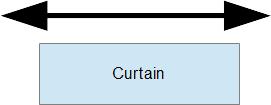
\includegraphics{curtainanalysis.png}
\caption{Curtain planar motion}
\end{figure}

\subsection{Door opening}
The opening of the door is a planar motion, with one degree of freedom. The degree of freedom is rotation about one axis of motion. The rotation should be limited, as in less than 90 degrees.
\begin{figure}[h!tb]
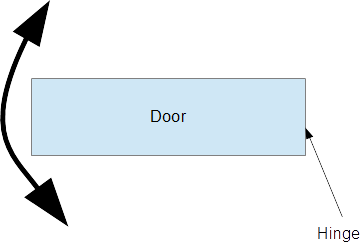
\includegraphics{dooranalysis.png}
\caption{Door planar motion}
\end{figure}

\subsection{Electrical Lights Arrangement}
The room is divided into portions and the lights multiplexed to allow efficient usage of the microcontroller's pins. Each portion of the room has an LDR at an optimum location and an LED associated with this portion. If the LDR does not detect enough light, the LED is lit. 

\section{Identification of the Structural Characteristics}
The material of choice was wood. This is because it is relatively cheap and easy to get. Basel was chosen because the simulation software used had all of its features and characteristics. The dimensions chosen are relatively smaller than the normal dimension of the objects to cater for the possibility of making a prototype.
\subsection{Curtain opening}
The mechanism will be relatively long and thin. Thin because it should not block the windows themselves. The length used is 65cm, and its maximum height should not be more than 10cm.
\\
Since window curtains have low weights,the mechanism should be able to withstand about 12kg. This value was got by assuming the maximum possible window curtain would be of 2m by 2m by 0.2cm dimensions and that the material it would be made of would be cotton (density 0f 1.5g / cm3).
\\
Its motion should not be noisy and opening and closing should occur relatively fast.\\
It should also have a means of attaching the curtain onto it.

\subsection{Door opening}
The mechanism should open a door 70cm long.
\\
The maximum weight to be supported during design is 20kg.
\\
Opening and closing should not be noisy and should occur relatively fast.
\\It should also have a means of attaching a door to it.

\subsection{Electrical Lights Arrangement}
The room is divided into 6 different portions each a different distance from the main window.

\section{Enumeration of Possible Kinematic Structures}
\subsection{Curtain opening}
For the curtain opening, since it is a simple translatory motion, the following means can be used to make the mechanism:
\subsubsection* {Cam and Follower}
A cam is a rotating machine element which gives reciprocating or oscillating motion to another element known as follower. The cam would be made such that the maximum distance travelled would be 70 cm, have a dwell to enable switching off, and have a return stroke of the same distance. However, this will result in a large cam and also the design will be complicated to cater for gravity {prevent follower from falling since the operations is in a horizontal direction).
\subsubsection* {Crank and slider}
A mechanism will be designed that receives rotary motion from a motor and translates it into linear motion using a 4 bar mechanism. The curtain will be attached to the slider.
\subsubsection* {Belt drive mechanism}
As the pulleys rotate, the belt moves in a linear motion. The curtain can be placed on the pulley and careful control of motor rotation made, such that opening and closing is achieved.

\subsection{Door opening}
Depending on the door design, it can be opened in various ways:

\subsubsection * {crank and rocker mechanism}
The crank receives the motor motion. Since the door is a hinge joint, the output link needs to rock through 90 degrees only otherwise breakage of the mechanism will occur.

\subsubsection* {Rack and pinion}
This will only work for sliding doors, whereby the door is connected to the pinion and the gears moves it back and forth.

\section{Sketching of Corresponding Mechanisms and Analyzing}
\subsection{Curtain opening}
\subsubsection* {Crank and slider}
The following 2D representation was done in linkage.
\begin{figure}[h!tb]
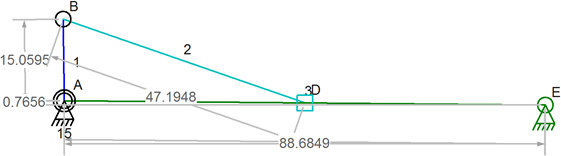
\includegraphics{curtainslider.jpg}
\caption{Slider mechanism as generated in Linkage}
\end{figure}

\subsubsection*{Belt drive mechanism}
The following 2D representation was done in SAM.
\begin{figure}[h!tb]
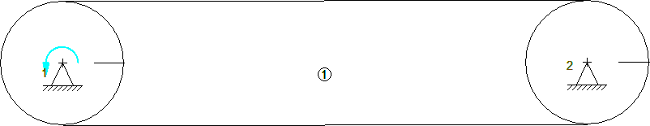
\includegraphics{belt.png}
\caption{Belt as generated in SAM61}
\end{figure}

\subsection{Door opening}
\subsubsection* (Crank and Rocker mechanism)
\begin{figure}[h!tb]
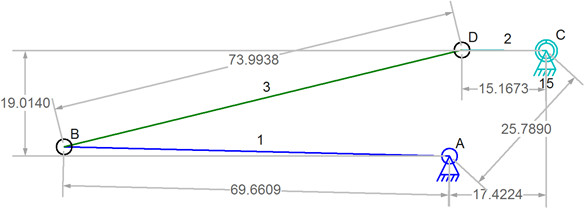
\includegraphics{doormechanism.jpg}
\caption{Door mechanism}
\end{figure}

\section{Selection of the Most Promision Mechanism}
For the curtain opening, slider mechanism. The belt mechanism would have been the best, but it would have been more expensive.
For the door opening, crank and rocker. This was because the main design was for a hinged door.
\section{Production phase}
Due to time constrains, this phase was not reached.

\chapter{Results and discussion}
Solid works was used to make the above mentioned mechanisms. Attached are the reports generated by solid works:
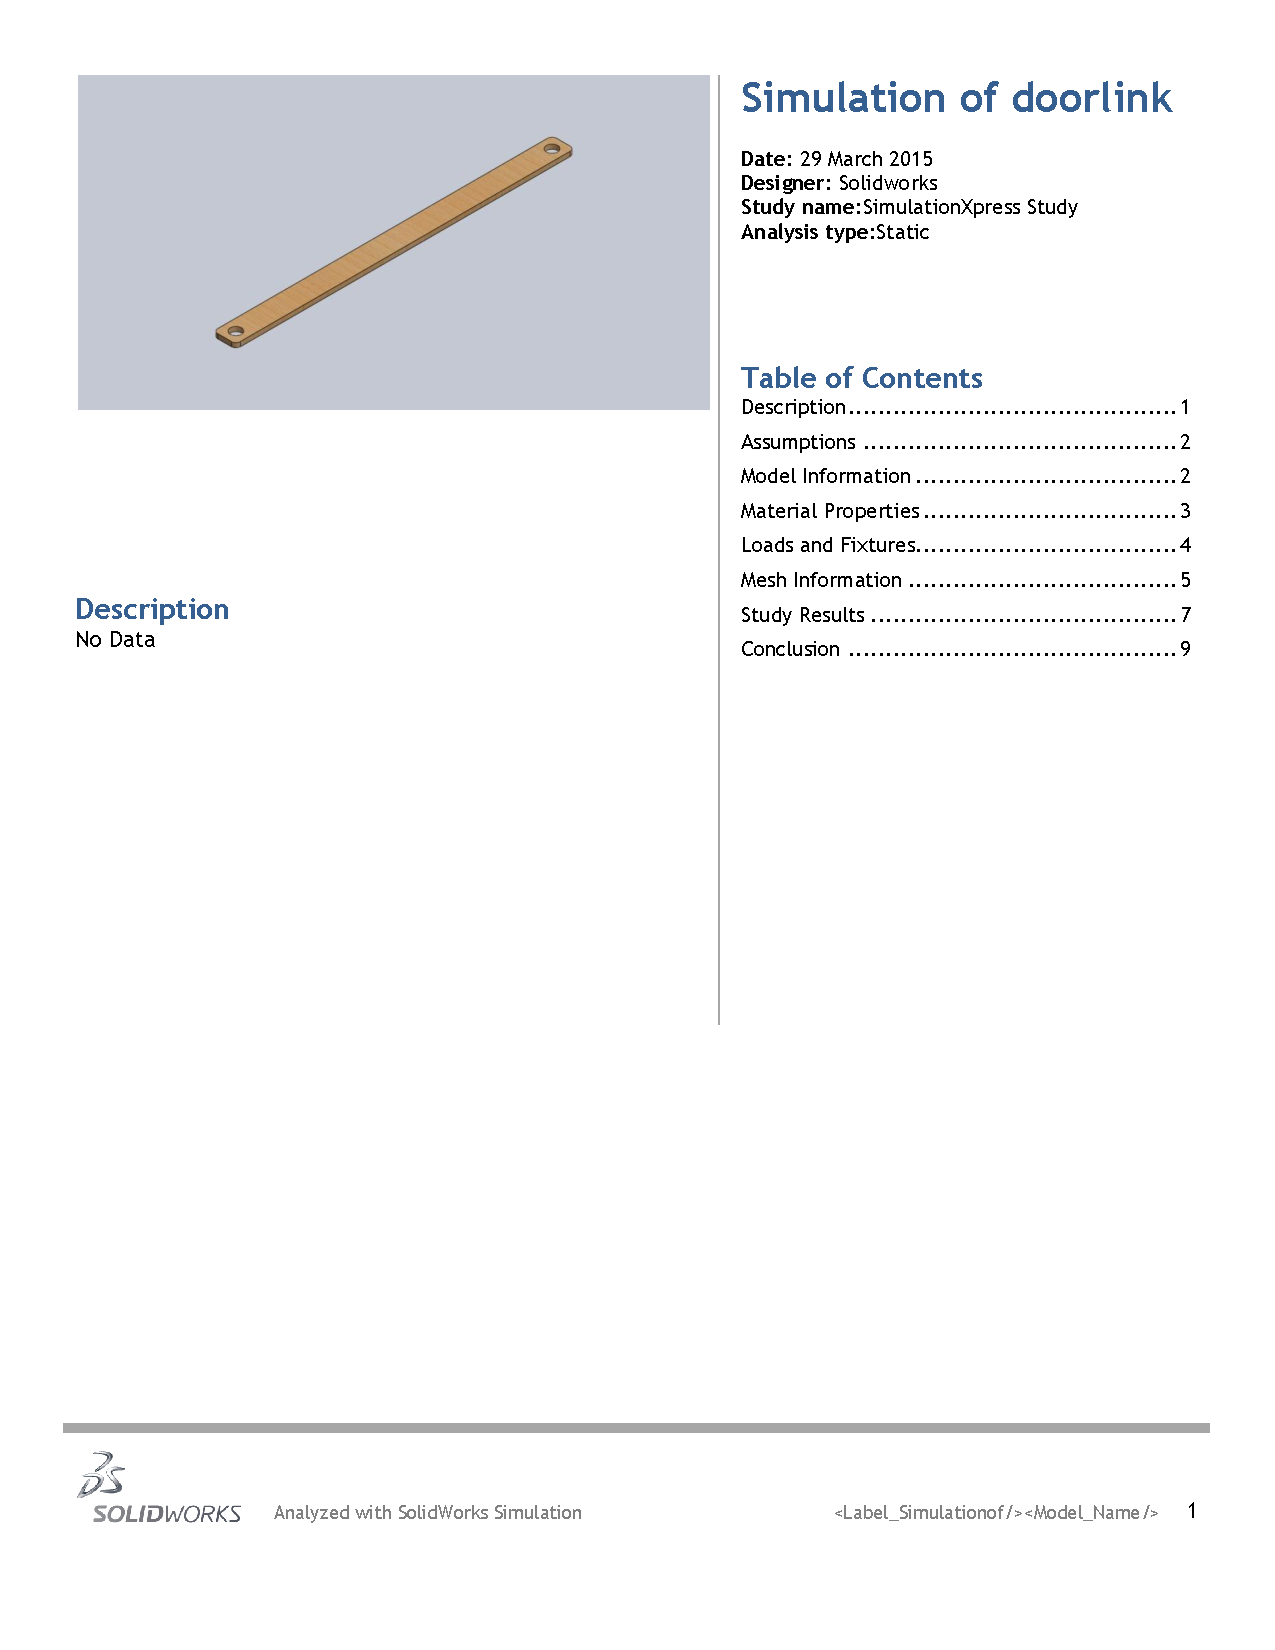
\includepdf[pages={-}]{doorlink_report.pdf}
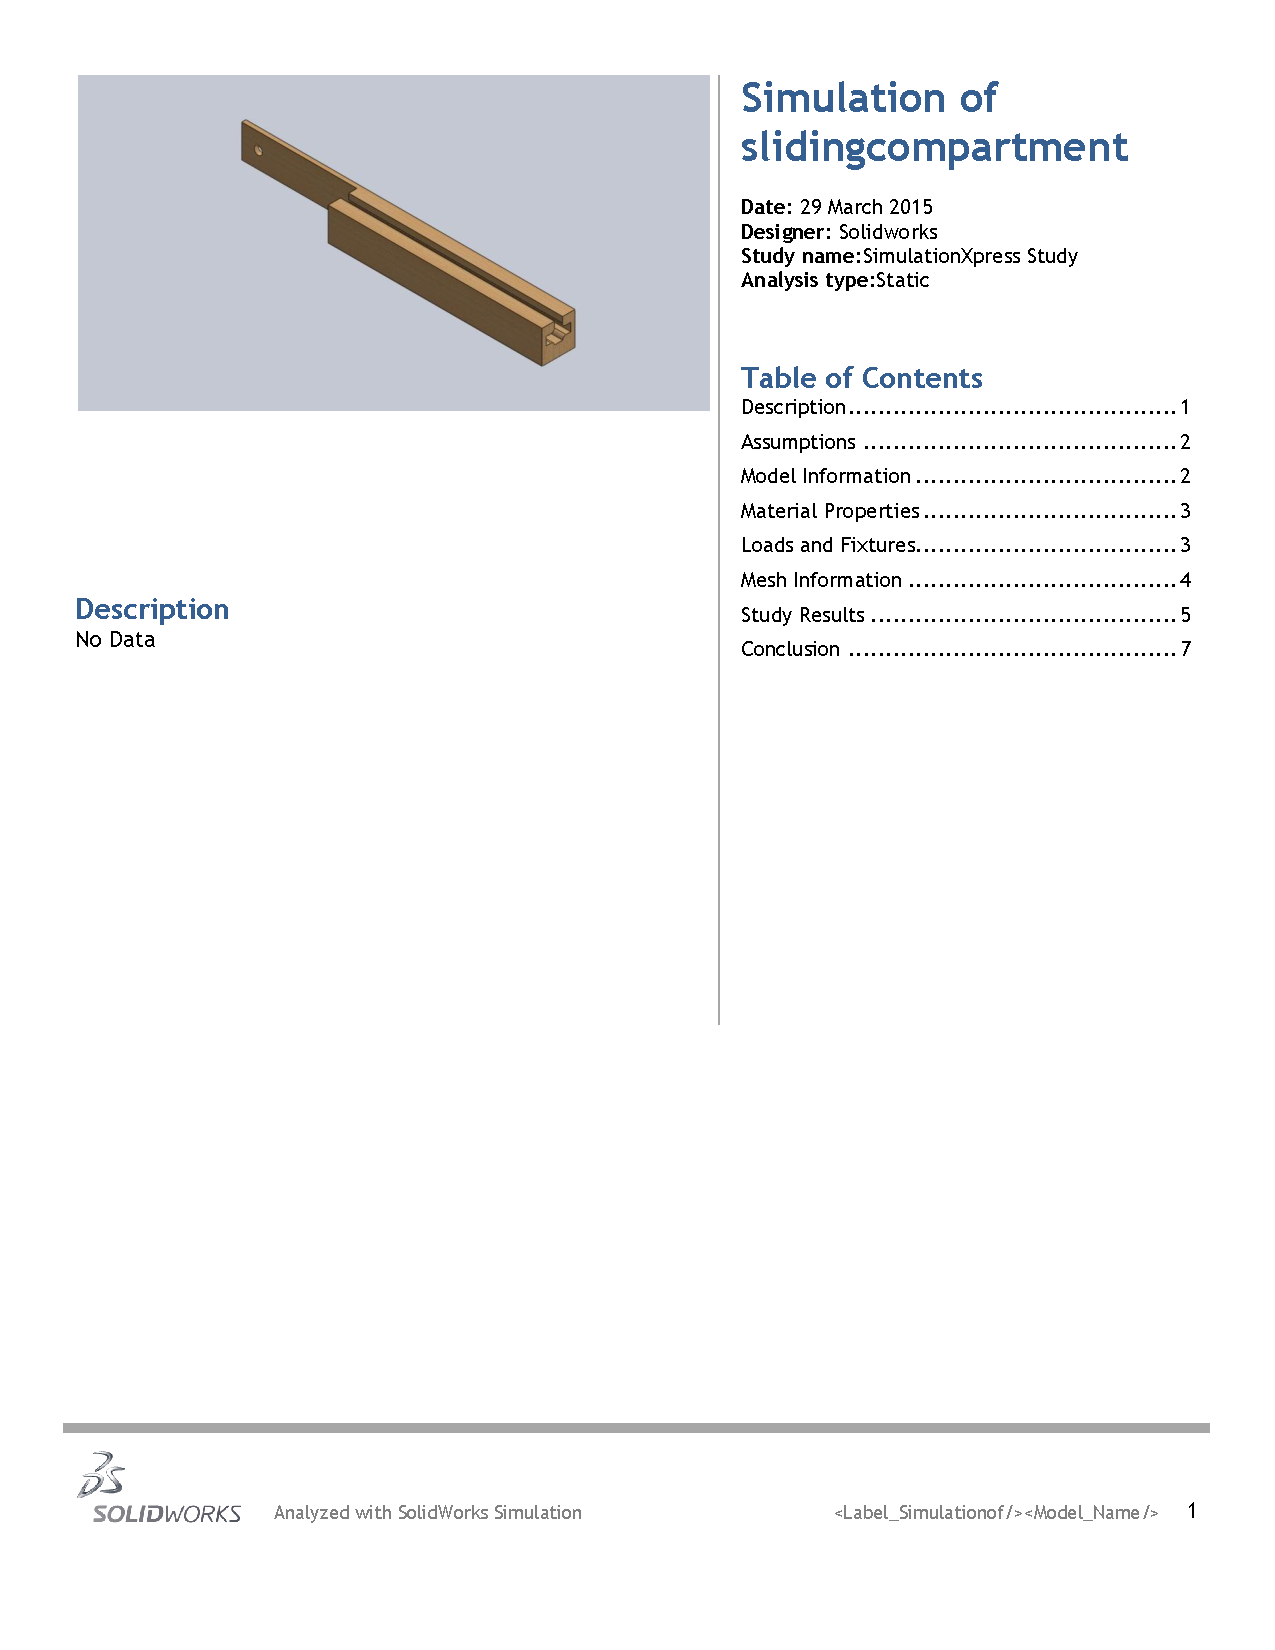
\includepdf[pages={-}]{slidingcompartment_report.pdf}

\chapter{Conclusion}


\begin{thebibliography}{9}
\bibitem{Tsai}Lung-Wen Tsai, Mechanism Design Enumeration of Kinematic Structures According to Function, CRC Press, 2001 

\end{thebibliography}

\end{document}
e 
